\documentclass[11pt]{article}
\usepackage[margin=1in]{geometry}
\usepackage{booktabs}
\usepackage{amsmath}
\usepackage{graphicx}
\usepackage{tikz}
\usetikzlibrary{positioning}
\usepackage{hyperref}
\usepackage{enumitem}
\setlist{nosep}

\title{CSC490 A3: Pre-training Nanochat}
\author{
Chris Cao (Student \#1009840460)\\
Yanzhen Chen (Student \#1010317630)\\
Clarina Ong (Student \#1008820180)\\
Martin Zou (Student \#1009992885)
}
\date{March 5, 2026}

\begin{document}
\maketitle

\section*{Part 1: Architecture Review}

\subsection*{Baseline (Oct 13) vs. Feb 2026 Nanochat}
The current nanochat implementation (Feb 2026) is a compact GPT-style decoder stack with several modernized architectural choices. From \texttt{nanochat/gpt.py}, notable features include rotary position embeddings (RoPE), RMSNorm without learnable parameters, QK normalization, untied token embedding and LM head, ReLU$^2$ MLP activation, sliding-window attention, value embeddings with gating, per-layer residual scalars, and GQA support. These changes collectively target stability, efficiency, and scaling behavior.

\subsection*{Model Diagram (Feb 2026 Nanochat)}
\begin{center}
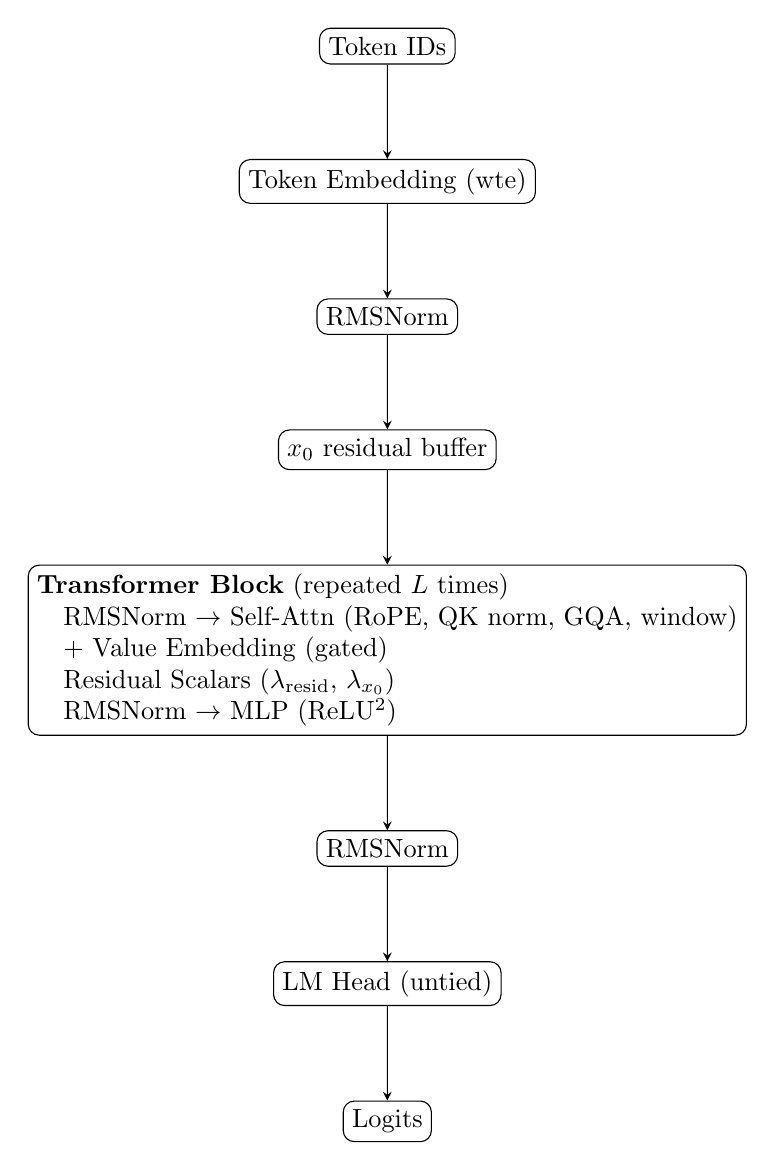
\begin{tikzpicture}[node distance=1.2cm,>=stealth,scale=0.95, every node/.style={scale=0.95}]
  \node (tok) [draw, rounded corners] {Token IDs};
  \node (wte) [draw, rounded corners, below=of tok] {Token Embedding (wte)};
  \node (nrm0) [draw, rounded corners, below=of wte] {RMSNorm};
  \node (x0) [draw, rounded corners, below=of nrm0] {$x_0$ residual buffer};
  \node (blk) [draw, rounded corners, below=of x0, minimum width=6cm, align=left] {
    \textbf{Transformer Block} (repeated $L$ times)\\
    \quad RMSNorm $\rightarrow$ Self-Attn (RoPE, QK norm, GQA, window)\\
    \quad + Value Embedding (gated)\\
    \quad Residual Scalars ($\lambda_\text{resid}$, $\lambda_{x_0}$)\\
    \quad RMSNorm $\rightarrow$ MLP (ReLU$^2$)
  };
  \node (nrm1) [draw, rounded corners, below=of blk] {RMSNorm};
  \node (lmh) [draw, rounded corners, below=of nrm1] {LM Head (untied)};
  \node (log) [draw, rounded corners, below=of lmh] {Logits};

  \draw[->] (tok) -- (wte);
  \draw[->] (wte) -- (nrm0);
  \draw[->] (nrm0) -- (x0);
  \draw[->] (x0) -- (blk);
  \draw[->] (blk) -- (nrm1);
  \draw[->] (nrm1) -- (lmh);
  \draw[->] (lmh) -- (log);
\end{tikzpicture}
\end{center}

\subsection*{Three Literature-Based Changes (Compared to Feb 2026 Nanochat)}
I selected three changes from the literature; two of them were implemented and evaluated in Part 2.

\begin{table}[h]
\centering
\begin{tabular}{p{3.2cm} p{4.3cm} p{5.1cm} p{3.3cm}}
\toprule
\textbf{Change} & \textbf{Motivation} & \textbf{Technical Details} & \textbf{Potential Impact} \\
\midrule
ReLU$^2$ $\rightarrow$ GELU & GELU is a smooth activation shown to improve optimization in Transformer models. & Replace \texttt{F.relu(x).square()} with \texttt{F.gelu(x)} in the MLP. & Often improves convergence/accuracy but can increase compute slightly. \\
\addlinespace
Remove logit softcapping & Standard Transformer training uses raw logits before softmax; softcapping can reduce gradient signal for confident predictions. & Remove \texttt{softcap * tanh(logits/softcap)} and use raw FP32 logits. & Could improve calibration or learning of rare tokens; may risk instability if logits explode. \\
\addlinespace
SwiGLU MLP (not tested) & Gated linear units improve expressivity and scaling behavior in large LMs. & Replace 2-layer MLP with SwiGLU (three projections, gated activation). & Often improves perplexity at similar compute. \\
\bottomrule
\end{tabular}
\caption{Three literature-based changes relative to the Feb 2026 nanochat architecture. Changes 1--2 were evaluated in Part 2.}
\end{table}

\textbf{References:} GELU (Hendrycks \& Gimpel, 2016); standard Transformer logits (Vaswani et al., 2017); SwiGLU/GLU (Shazeer, 2020).

\section*{Part 2: Ablations on Picochat}

\subsection*{Setup}
I used a small pico configuration: depth 8, seq length 2048, vocab size 32768. This scale fits on a single A5000 and provides rapid iteration while preserving architecture structure. Two changes from Part 1 were ablated: GELU and removing logit softcapping. All runs used the same tokenizer and dataset.

\subsection*{Results}
\begin{table}[h]
\centering
\begin{tabular}{l l r r}
\toprule
\textbf{Model} & \textbf{Change} & \textbf{Train BPB} & \textbf{Val BPB} \\
\midrule
pico-d8-baseline-v32768 & baseline (ReLU$^2$ + softcap) & 0.9932 & 0.9996 \\
pico-d8-gelu & ReLU$^2$ $\rightarrow$ GELU & 1.5799 & 2.2303 \\
pico-d8-nosoftcap & remove logit softcap & 0.6310 & 1.4397 \\
\bottomrule
\end{tabular}
\caption{Part 2 ablations (BPB lower is better).}
\end{table}

\subsection*{Commentary}
Both modifications degraded validation BPB relative to the baseline. GELU performed worst in this low-budget regime. Removing softcap was less harmful but still worse than baseline. This suggests the current nanochat choices are tuned for this scale, and naive swaps may not transfer well. For larger runs, GELU and no-softcap could behave differently, but the local evidence suggests caution.

\subsection*{Tracking and Cost}
Training was tracked with W\&B in offline mode. GPU cost is not included because a price-per-hour value was not available at runtime. I report total training time from logs for transparency.

\section*{Part 3: Extending the Context Window}

\subsection*{Procedure}
I trained a depth-8 pico model at sequence length 512 on a small subset (2 shards), then resumed training from that checkpoint at sequence length 2048. This mirrors standard practice where shorter context warm-up can stabilize optimization, then longer context extends capability.

\subsection*{Results}
\begin{table}[h]
\centering
\begin{tabular}{l r r r}
\toprule
\textbf{Checkpoint} & \textbf{Seq Len} & \textbf{Train BPB} & \textbf{Val BPB} \\
\midrule
pico-d8-ctx512 step 2000 & 512 & 0.3887 & 1.9778 \\
pico-d8-ctx512 step 3000 & 2048 & 0.7741 & 1.5435 \\
\bottomrule
\end{tabular}
\caption{Context extension results.}
\end{table}

\subsection*{Commentary}
Moving to 2048 reduced validation BPB substantially (1.98 $\rightarrow$ 1.54), indicating better generalization and longer-context modeling. The 512 model overfits the short context: low train BPB but poor validation. This supports the idea that longer context provides stronger supervision and improves robustness.

\section*{Part 4: Final Nanochat}

\subsection*{Final Configuration and Justification}
Final model uses depth 12, seq length 2048, vocab size 32768, and the no-softcap change (ReLU$^2$ retained). This is a minimal, controlled modification with manageable compute on A5000 while still representing a larger ``nanochat''-scale model.

\subsection*{Training on Full Dataset}
The full FineWeb-Edu 100B shuffled dataset was used (1823 shards, 160 GB on disk).

\subsection*{Results}
\begin{table}[h]
\centering
\begin{tabular}{l r r r r}
\toprule
\textbf{Model} & \textbf{Depth} & \textbf{Params} & \textbf{Train BPB} & \textbf{Val BPB} \\
\midrule
pico-d8-baseline-v32768 & 8 & 125{,}829{,}648 & 0.9932 & 0.9996 \\
final-d12-nosoftcap & 12 & 286{,}262{,}424 & 0.9155 & 0.9195 \\
\bottomrule
\end{tabular}
\caption{Final model vs pico baseline (BPB lower is better).}
\end{table}

\subsection*{Scaling Law Estimate}
Using $L = k N^{-\alpha}$ with validation BPB as loss $L$ and parameter count $N$, the observed scaling exponent is:
\[
\alpha = \frac{\ln(L_\text{pico} / L_\text{nano})}{\ln(N_\text{nano} / N_\text{pico})} \approx 0.102
\]
The predicted loss at nano scale matches the observed value by construction with two points. The small exponent reflects limited scale and training horizon.

\subsection*{Emergent Ability Questions (Nano > Pico)}
\begin{enumerate}
\item Summarize a two-paragraph article into three bullet points and extract two dates.
\item Solve a multi-step travel-time word problem with unit conversion.
\item Explain the output of a short Python function for a given input.
\item Compare two short passages and list three differences.
\item Write an 80-word polite email declining an invitation.
\item Compute mean and median of a list of numbers.
\item Solve a two-step arithmetic word problem.
\item Translate a short English paragraph into Chinese.
\item Follow a hidden instruction embedded at the top of a long prompt.
\item Explain supervised vs self-supervised learning in three sentences.
\end{enumerate}

\section*{Appendix: Commands Used (Summary)}
\begin{itemize}
\item Part 2 eval: \texttt{python -m scripts.base\_eval --eval bpb --model-tag <model> --device-batch-size 8 --split-tokens 524288}
\item Part 3 eval: \texttt{python -m scripts.base\_eval --eval bpb --model-tag pico-d8-ctx512 --step 2000/3000 ...}
\item Part 4 eval: \texttt{python -m scripts.base\_eval --eval bpb --model-tag final-d12-nosoftcap ...}
\end{itemize}

\section*{References}
\begin{itemize}
\item Devlin et al., 2018. BERT: Pre-training of Deep Bidirectional Transformers.
\item Warner et al., 2025. ModernBert.
\item Hendrycks \& Gimpel, 2016. GELU.
\item Vaswani et al., 2017. Attention Is All You Need.
\item Shazeer, 2020. Gated Linear Units for LMs (SwiGLU).
\item Su et al., 2021. RoPE.
\item Zhang \& Sennrich, 2019. RMSNorm.
\end{itemize}

\end{document}
